\documentclass[a4paper,12pt]{article}

\usepackage{ucs}
\usepackage[utf8x]{inputenc}
\usepackage[russian]{babel}
%\usepackage{cmlgc}
\usepackage{graphicx}
\graphicspath{ {./images/} }
\usepackage{listings}
\usepackage{xcolor}
% \usepackage{hyperref}
% \hypersetup{
%     colorlinks=true,
%     linkcolor=black,
%     filecolor=black,      
%     urlcolor=cyan,
%     pdftitle={НИР},
%     pdfpagemode=FullScreen,
%     }
\usepackage{float}
%\usepackage{courier}


% для поддержки джаваскрипта. сурс - tex.stackexchange.com %
% \usepackage{color}
% \definecolor{lightgray}{rgb}{.95,.95,.95}
% \definecolor{darkgray}{rgb}{.4,.4,.4}
% \definecolor{purple}{rgb}{0.53, 0.26, 0.75}
% \definecolor{maroon}{rgb}{0.7, 0.24, 0.2}
% \definecolor{cobalt}{rgb}{0.03, 0.44, 0.73}
% \lstdefinelanguage{JavaScript}{
%   keywords={break, case, catch, continue, debugger, default, delete, do, else, false, finally, for, function, if, in, instanceof, new, null, return, switch, this, throw, true, try, typeof, var, void, while, with},
%   morecomment=[l]{//},
%   morecomment=[s]{/*}{*/},
%   morestring=[b]',
%   morestring=[b]»,
%   ndkeywords={class, export, boolean, throw, implements, import, this},
%   keywordstyle=\color{cobalt}\bfseries,
%   ndkeywordstyle=\color{darkgray}\bfseries,
%   identifierstyle=\color{black},
%   commentstyle=\color{purple}\ttfamily,
%   stringstyle=\color{maroon}\ttfamily,
%   sensitive=true
% }

% \lstset{
%    language=JavaScript,
%    backgroundcolor=\color{lightgray},
%    extendedchars=true,
%    basicstyle=\footnotesize\ttfamily,
%    showstringspaces=false,
%    showspaces=false,
%    numbers=left,
%    numberstyle=\footnotesize,
%    numbersep=9pt,
%    tabsize=2,
%    breaklines=true,
%    showtabs=false,
%    captionpos=b
% }

\makeatletter
\renewcommand\@biblabel[1]{#1.}
\makeatother

\newcommand{\myrule}[1]{\rule{#1}{0.4pt}}
\newcommand{\sign}[2][~]{{\small\myrule{#2}\\[-0.7em]\makebox[#2]{\it #1}}}

% Поля
\usepackage[top=20mm, left=30mm, right=10mm, bottom=20mm, nohead]{geometry}
\usepackage{indentfirst}

% Межстрочный интервал
\renewcommand{\baselinestretch}{1.50}


\begin{document}

%%%%%%%%%%%%%%%%%%%%%%%%%
%%%                   %%%
%%% Титульный лист    %%%

\thispagestyle{empty}
\begin{center}


\renewcommand{\baselinestretch}{1}
{\large
{\sc Петрозаводский государственный университет\\
Институт математики и информационных технологий\\
	Кафедра Информатики и Математического Обеспечения
}
}

\end{center}


\vfill

\begin{center}
{\normalsize Отчет о практике по научно-исследовательской работе} \\

\medskip

%%% Название работы %%%
	{\Large \sc Разработка CRM-системы для компании «МастерЛОС»} \\
    (промежуточный)
\end{center}

\medskip
\normalsize
\renewcommand{\baselinestretch}{1.2}
\begin{flushright}
\parbox{11cm}{%
Выполнила:\\
студентка 4 курса группы 22405\\
С. Э. Зименкова 
\begin{flushright}
\sign[подпись]{4cm}
\end{flushright}

Место прохождения практики: \\ Кафедра Информатики и Математического Обеспечения\\

Период прохождения практики: \\ 02.09.24-15.12.24


Научный руководитель:\\
%%% степень, звание ФИО научного руководителя %%%
% Первый руководитель 
Д. Б. Чистяков \\
\begin{flushright}
\sign[подпись]{4cm}
\end{flushright}

Итоговая оценка \\
\begin{flushright}
\sign[оценка]{4cm}
\end{flushright}

% Второй руководитель 
% И. О. Фамилия, ученая степень, ученое звание \\
% \begin{flushright}
% \sign[подпись]{4cm}
% \end{flushright}
}
\end{flushright}

\vfill

\begin{center}
\large
    Петрозаводск --- 2024
\end{center}

%%% Титульный лист    %%%
%%%                   %%%
%%%%%%%%%%%%%%%%%%%%%%%%%


%%%%%%%%%%%%%%%%%%%%%%%%%
%%%                   %%%
%%% Содержание        %%%

\newpage

\tableofcontents

%%% Содержание        %%%
%%%                   %%%
%%%%%%%%%%%%%%%%%%%%%%%%%


%%%%%%%%%%%%%%%%%%%%%%%%%
%%%                   %%%
%%% Введение          %%%

\newpage
\section*{Введение}
\addcontentsline{toc}{section}{Введение}
Магазин «МастерЛОС» занимается поставкой и установкой автономного очистного оборудования для физических и юридических лиц. Специалисты компании подбирают подходящее оборудование на основании обследования земельного участка, поставляют и устанавливают водопровод и очистные сооружения. Также компания предоставляет регулярное сервисное обслуживание установленного оборудования. Компания работает с 2009 года и обеспечивает гарантийное и послегарантийное обслуживание, является официальным поставщиком компаний-производителей оборудования.

Директор магазина «Мастер ЛОС» выступает в качестве Заказчика программного продукта для автоматизации процессов, связанных с взаимодействием клиентов. За срок работы магазина накопилась достаточно большая база данных клиентов, однако процесс взаимодействия с покупателями, контроля регулярного обслуживания оборудования и остатков оборудования на складе не автоматизирован, а учет ведется только в формате разрозненных электронных таблиц. Подобный способ ведения учета стал снижать эффективность работы сотрудников магазина.

Для решения этой проблемы было решено внедрить в работу магазина автоматизированную систему для управления взаимоотношениями с клиентами, которая поможет сотрудникам централизованно хранить всю информацию о клиентах, а также поможет контролировать склад оборудования, текущие работы по клиентам и регулярное сервисное обслуживание.

Цель данной работы --- разработать и внедрить автоматизированную информационную систему для управления процессами Заказчика. В настоящий момент системе присвоено сокращенное название «Мастер CRM».

Для осуществления поставленной цели необходимо выполнить следующие задачи:
\begin{enumerate}
    \item Провести обследование процессов предприятия Заказчика;
    \item Сформулировать техническое задание на разработку системы;
    \item Создать макет дизайна автоматизированной системы;
    \item Разработать и протестировать программный код автоматизированной системы;
    \item Внедрить автоматизированную систему на предприятие заказчика;
    \item Исправить найденные в процессе эксплуатации недочеты и поддерживать работу системы в будущем.
\end{enumerate}

%%% Введение          %%%
%%%                   %%%
%%%%%%%%%%%%%%%%%%%%%%%%%


%%%%%%%%%%%%%%%%%%%%%%%%%
%%%                   %%%
%%% Глоссарий         %%%

\newpage
\section*{Глоссарий}
\addcontentsline{toc}{section}{Глоссарий}

База данных компании --- набор таблиц, не объединенных никакой СУБД. Директор и менеджеры используют термин «База данных» в описании всех таблиц в совокупности несмотря на то, что они не объединены каким-либо алгоритмом.

Таблица --- документ формата .xlsx, т.е. книга Excel, или документ Google Sheets.

Оборудование --- любое средство, устанавливаемое на участке клиента: септики, очистные станции, водопроводные трубы, ливневые канализации и так далее.

АИС --- Автоматизированная Информационная Система.

CRM --- англ. Customer Relationship Management, система управления взаимоотношений с клиентами.


%%% Глоссарий         %%%
%%%                   %%%
%%%%%%%%%%%%%%%%%%%%%%%%%


%%%%%%%%%%%%%%%%%%%%%%%%%
%%%                   %%%
%%% Глава 1           %%%

\newpage
\section{Анализ предметной области}
\subsection{Структура организации}
Во главе организации находится директор магазина. В его подчинении находятся три подразделения (см. Рис. \ref{fig:company_structure})
\begin{itemize}
    \item Отдел продаж
    \item Бухгалтерия
    \item Сервисный центр
\end{itemize}

Отдел продаж занимается общением с клиентами, заключением сделок, оформлением документов продажи, а также контролем остатков товаров на складе и заказом недостающих позиций. В структуру отдела продаж входят менеджеры по продажам.

Бухгалтерия ведет бухгалтерский учет, предоставляет отчетность в налоговые органы. Бухгалтерией руководит главный бухгалтер.

Сервисный центр осуществляет работы по осмотру земельных участков, подбору оборудования, установке систем, сервисному обслуживанию. В структуру сервисного центра входят мастера, монтажники и сервис-инженеры под руководством начальника сервисного центра (мастера).

\begin{figure}[H]
    \centering
    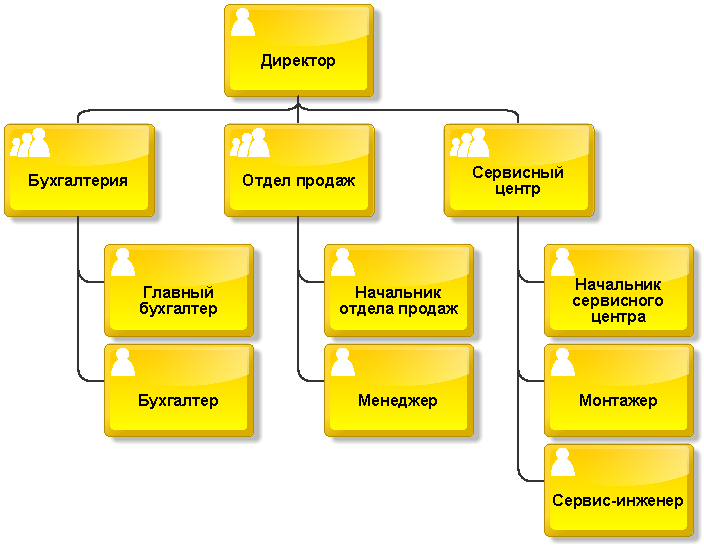
\includegraphics[width=0.8\linewidth]{company_structure.png}
    \caption{Структура управления}
    \label{fig:company_structure}
\end{figure}

\subsection{Цель деятельности}
Главной целью деятельности магазина является получение прибыли путем продажи и установки оборудования клиентам (физическим и юридическим лицам).

\subsection{Миссия и стратегия компании}
Миссия компании --- создавать комфорт и безопасность для клиентов, обеспечивая их качественными, надежными и экологичными решениями для автономных очистных систем; сделать установку и обслуживание локальных очистных сооружений доступным и удобным процессом, приносящим спокойствие и уверенность в надежности системы на долгие годы.

Для достижения миссии компания «МастерЛОС» ставит перед собой следующие цели и задачи:
\begin{itemize}
    \item Высокий уровень клиентского сервиса
    \begin{itemize}
        \item Качественные бесплатные консультации: клиенты получают всю необходимую информацию о вариантах и стоимости оборудования и его установки.
        \item Индивидуальный подход: для каждого клиента проводится бесплатный выезд и обследование участка с учетом существующей инфраструктуры, чтобы предложить оптимальное решение.
        \item Прозрачность процессов: весь процесс взаимодействия с клиентом сопровождается четким и своевременным информированием клиента, понятным ценообразованием и ясностью в этапах работы.
    \end{itemize}
    \item Гарантия качества и надежности оборудования
    \begin{itemize}
    \item Поддержка отношений с надежными поставщиками и регулярная оценка качества типового и нетипового оборудования.
    \item Строгий контроль процесса установки на каждом этапе: специалисты компании четко следуют сформированному плану работ и контролируют качество выполнения каждого шага.
    \end{itemize}
    \item Профессионализм команды и высокая скорость обслуживания
    \begin{itemize}
        \item Повышение навыков сотрудников за счет обучения и повышения квалификации.
        \item Автоматизация таких процессов, как контроль работ по заказу клиента, складской учет, контроль регулярных сервисных работ.
    \end{itemize}
    \item Поддержание долгосрочных отношений с клиентами через систему регулярного обслуживания
    \begin{itemize}
        \item Информирование клиентов о необходимости регулярного обслуживания, выбор частоты обслуживания индивидуально для каждого клиента
        \item Поддержка надежной работы оборудования на протяжении всего срока службы, обеспечение гарантии стабильного функционирования системы.
    \end{itemize}
    \item Поддержка экологических и инновационных решений
    \begin{itemize}
        \item Подбор современного и экологического оборудования для клиентов: поставка систем, которые снижают энергопотребление и нагрузку на окружающую среду.
    \end{itemize}
\end{itemize}

Стратегия компании представлена на Рис. \ref{fig:company_strategy}

\begin{figure}[H]
    \centering
    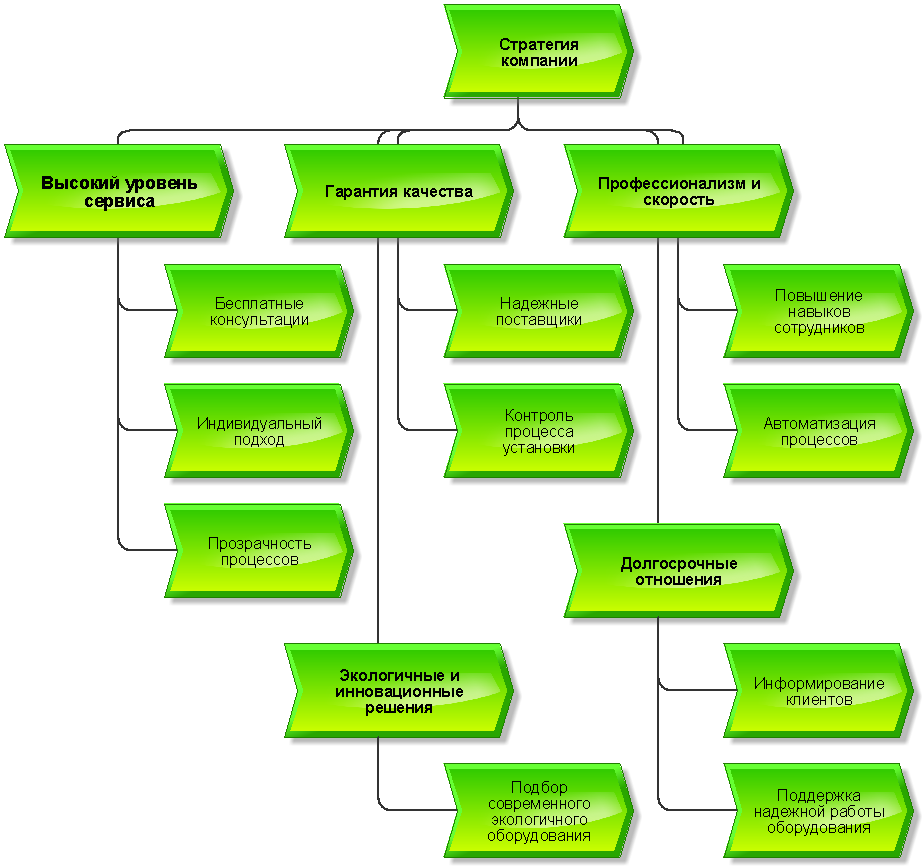
\includegraphics[width=0.8\linewidth]{company_strategy.png}
    \caption{Стратегия компании}
    \label{fig:company_strategy}
\end{figure}

\subsection{Виды деятельности компании}
К основным видам деятельности компании относятся:
\begin{itemize}
    \item Продажа и установка оборудования
    \item Обслуживание и консультирование
\end{itemize}

Вспомогательным видом деятельности является поддержание остатков товара на складе.

\subsection{Описание бизнес-процессов}
В ходе исследования компании были выделены и изучены следующие бизнес-процессы:
\begin{enumerate}
    \item Предпродажная работа
    \item Выполнение заказа клиента
    \item Регулярное обслуживание оборудования
    \item Заказ оборудования у поставщика
\end{enumerate}

\subsubsection{Описание БП «Предпродажная работа»}

Предпродажные работы выполняются сотрудниками компании бесплатно в целях заинтересовать клиента предложением. Процесс начинается с обращения клиента в компанию по номеру телефона.

\begin{enumerate}
    \item Менеджер принимает звонок клиента и выясняет, работал ли клиент ранее с компанией, если клиент обращается впервые --- задает основные вопросы (ФИО, контактные данные, адрес проведения работ).
    \item Далее менеджер уточняет у клиента основную информацию о запросе и передает запрос клиента начальнику сервисного центра (для краткости принято называть начальника сервисного центра «мастером»).
    \item Мастер связывается с клиентом, чтобы договориться о бесплатном сервисном выезде на участок клиента. Выезд осуществляется с целью провести анализ участка работ, подробно расспросить клиента о его пожеланиях, озвучить примерную стоимость и заполнить опросный лист.
    \item После осмотра участка мастер возвращается в офис компании, формирует смету на оборудование и работы по установке, передает смету менеджеру.
    \item Менеджер общается с клиентом по смете: озвучивает стоимости и условия, отрабатывает возражения.
    \item Если в результате предпродажных работ клиент согласен на поставку и установку оборудования, происходит переход к бизнес-процессу «Выполнение заказа клиента», иначе договор не заключается и работы не выполняются.
\end{enumerate}

Диаграмма процесса приведена в Приложении, см. Рис. \ref{fig:pred1}, \ref{fig:pred2}.

\subsubsection{Описание БП «Выполнение заказа клиента»}

\begin{enumerate}
    \item Если клиент соглашается на поставку и установку оборудования, менеджер подготавливает договор и счет на предоплату.
    \item Клиент проверяет, что вся информация в договоре указана верно, подписывает договор и оплачивает счет.
    \item Менеджер передает мастеру информацию о заказе, мастер согласовывает сроки выполнения работ с клиентом.
    \item Мастер и монтажная бригада выполняют работы по установке оборудования по договору, мастер передает клиенту техпаспорт оборудования, клиент подписывает закрывающие документы (акты).
    \item Мастер передает документы менеджеру. Менеджер выставляет клиенту счет на дооплату и уточняет, как часто клиент планирует пользоваться оборудованием. В зависимости от того, какой ответ даст клиент (круглый год, полгода, только летом, несколько раз в год), менеджер укажет соответствующую периодичность обслуживания в таблице.
    \item Клиент оплачивает счет, сообщает, насколько часто планирует пользоваться оборудованием. 
    \item Менеджер рассчитывает, как часто оборудованию потребуется регулярное обслуживание, отмечает эту информацию в таблице, и клиент переводится на обслуживание.
\end{enumerate}
       
Диаграмма процесса приведена в Приложении, см. Рис. \ref{fig:exec1}, \ref{fig:exec2}. Для упрощения читаемости диаграммы монтажная команда как отдельный исполнитель была опущена. 

\subsubsection{Описание БП «Заказ оборудования у поставщика»}

Процесс заказа оборудования у поставщика делится на два подпроцесса: заказ типового оборудования по мере уменьшения остатка на складе и заказ нетипового оборудования по заказу клиента.

Заказ типового оборудования инициируется по мере расходования остатка на складе:

\begin{enumerate}
    \item Менеджер записывает текущий остаток оборудования на складе и его изменение при выполнении заказов клиентов, и когда на складе остается мало какой-либо из позиций, менеджер сообщает об этом директору.
    \item Директор связывается с поставщиком типового оборудования, передает ему список необходимых позиций и их количество, запрашивает счет на оплату.
    \item После получения и оплаты счета компанией поставщик направляет оборудование на склад компании.
    \item После осуществления доставки поставщик передает эту информацию директору, директор осуществляет контроль качества поставки и передает информацию о доставленных позициях менеджеру.
    \item Менеджер актуализирует информацию о количестве каждой закупленной позиции в таблице.
\end{enumerate}

Заказ нетипового оборудования происходит при необходимости установить нетиповое оборудование конкретному клиенту:

\begin{enumerate}
    \item Мастер в процессе предпродажных работ составляет смету и передает ее менеджеру.
    \item Если в результате предпродажных работ клиент подписывает договор, менеджер инициирует заказ нетипового оборудования.
    \item Менеджер передает информацию о необходимости заказать нетиповое оборудование директору, который связывается с производителем оборудования и просит выставить счет на изготовление.
    \item После получения и оплаты счета компанией производитель изготавливает оборудование и отправляет его на склад компании.
    \item Производитель уведомляет директора, директор принимает доставку оборудования и передает информацию мастеру.
    \item Мастер проверяет целостность доставленного оборудования и переходит к выполнению заказа клиента.
\end{enumerate}

Диаграмма процесса приведена в Приложении, см. Рис. \ref{fig:order1}, Рис. \ref{fig:order2}.


\subsubsection{Описание БП «Регулярное обслуживание оборудования»}

После установки оборудования клиенту необходимо с определенной периодичностью осуществлять регулярное сервисное обслуживание. В зависимости от того, как часто клиент пользуется системой, менеджер определяет период обслуживания. Например, если в частном доме установлена скважина и очистная станция, и семья живет в этом доме круглый год, сервисное обслуживание нужно проводить не реже, чем раз в 6 месяцев.

\begin{enumerate}
    \item Менеджер регулярно проверяет, каким клиентам требуется обслуживание оборудования.
    \item Поскольку часто ситуация, озвученная клиентом при установке, отличается от реальной, менеджер связывается с клиентом и уточняет, требуется ли ему сервисное обслуживание.
    \item Если клиент сообщает, что пользовался оборудованием реже, чем планировал при установке (например, долго не мог достроить дом, и система не использовалась, или не стал оставаться на даче на зиму и переехал в город), менеджер определяет новую дату обслуживания и записывает ее в базу данных, чтобы связаться с клиентом позже.
    \item Если клиент подтверждает, что система использовалась согласно плану, менеджер записывает информацию о необходимости обслуживания, передает ее начальнику сервисного центра (мастеру).
    \item Мастер согласовывает дату и время обслуживания.
    \item Далее процесс осуществляется аналогично процессу выполнения заказа клиента.
\end{enumerate}

Диаграмма процесса приведена в Приложении, см. Рис. \ref{fig:service}.

\subsection{Результаты исследования}

В результате общения с сотрудниками компании «МастерЛОС» и исследования бизнес-процессов компании было установлено, что недостаток организации и отсутствие автоматизированной системы для контроля процессов приводит к снижению эффективности работы сотрудников.

\subsubsection{Проблемы, выявленные при исследовании функций организации}

Выявленные недостатки процессов включают:
\begin{itemize}
    \item Обмен важной информацией между сотрудниками через электронную почту, личное общение, телефонные звонки и мессенджеры может привести к утере информации и нарушению сроков выполнения задач, хотя и кажется более быстрым, чем регистрация документов и заказов в какой-либо системе.
    \item Использование нескольких разрозненных таблиц формата Excel или Google Sheets вместо централизованного хранения информации в общей базе данных может привести к рассинхронизации информации между таблицами и между устройствами сотрудников.
    \item Директор привлекается к выполнению процессов, не связанных с управлением компании: запрашивает счета у поставщиков, принимает доставку товаров. Это повышает рабочую нагрузку на директора, который не должен заниматься логистикой или выполнением работ, поскольку эти задачи могут выполняться другими сотрудниками или автоматически.
    \item Обеспечение регулярного обслуживания оборудования клиентов выполняется только при ручном контроле сроков со стороны менеджера. Поскольку в процессе не используется какое-либо ПО или другое средство, осуществляющее автоматический контроль сроков обслуживания и уведомляющее менеджера о необходимости связаться с клиентом, это может привести к пропуску сервисного обслуживания или несвоевременному выполнению сервисного обслуживания.
    \item Своевременный заказ заканчивающихся позиций на складе осуществляется только при ручном контроле остатков со стороны менеджера, при этом ввод изменений в остатке тоже осуществляется вручную и может привести к расхождению между реальным остатком на складе и зарегистрированным в таблице количеством. Это может привести к несвоевременному заказу оборудования и задержкам в процессе выполнения заказа клиента, что понижает удовлетворение клиента работой компании и ухудшает имидж компании.
\end{itemize}

\subsubsection{Первичные требования Заказчика к внедряемой системе}

Для решения перечисленных проблем Заказчик желает внедрить в процессы компании использование автоматизированной системы. Система должна содержать в себе централизованную базу данных, предоставлять инструменты для хранения и обмена важной информацией между сотрудниками, автоматически контролировать отгрузку, поступление и остаток позиций на складе, напоминать менеджеру о необходимости сервисного обслуживания для всех клиентов. Также рекомендуется исключить необходимость привлечения директора к рабочему процессу, за исключением согласования оплаты счетов и спорных моментов.

%%% Глава 1           %%%
%%%                   %%%
%%%%%%%%%%%%%%%%%%%%%%%%%



%%%%%%%%%%%%%%%%%%%%%%%%%
%%%                   %%%
%%% Глава 2           %%%

\newpage
\section{Техническое задание}
В настоящий момент сформулировано высокоуровневое техническое задание на разработку АИС «Мастер CRM».

\subsection{Цели создания системы}

Основными целями внедрения системы являются:
\begin{itemize}
    \item Оптимизация процесса взаимодействия менеджера с клиентом;
    \item Упрощение оперативной регистрации и отслеживания этапа работ по заказу клиента;
    \item Упрощение контроля остатков товаров на складе;
    \item Перевод документооборота, ведущегося в виде разрозненных файлов в разных системах, в единую информационную систему;
    \item Повышение качества принятия управленческих решений за счет оперативности представления и удобства отображения информации;
    \item Предоставление сотрудникам компании доступа к системе с любого устройства, имеющего доступ в Интернет, вне зависимости от расположения.
\end{itemize}


\subsection{Общие требования к структуре и функционированию системы}

АИС «Мастер CRM» должна быть реализована в виде веб-сайта, расположенного на сервере в защищенном от несанкционированного доступа и пригодном для безопасной и стабильной работы электрооборудования помещении в офисе магазина. Электронно-вычислительная техника и публичный IP-адрес, необходимые для расположения сервера системы в офисе, предоставляются Заказчиком. 

Работа пользователя с системой должна осуществляться посредством графического интерфейса в веб-браузере на персональном компьютере или мобильном устройстве. Графический интерфейс должен обладать следующими свойствами:
\begin{enumerate}
    \item Соответствие современным эргономическим требованиям и обеспечение удобного доступа к основным функциям и операциям системы;
    \item Управление с помощью набора экранных меню, кнопок, значков и других элементов;
    \item Простота и удобство использования;
    \item Все надписи экранных форм, а также сообщения, выдаваемые пользователю (кроме системных сообщений) должны быть на русском языке;
    \item Должен быть выполнен в едином графическом дизайне, приятном для восприятия и повторяющем дизайн веб-сайта компании.
\end{enumerate}

Поскольку система содержит информацию о клиентах компании и важную информацию, утеря которой будет критична для продолжения работы магазина, система должна иметь подсистему защиты.\\

Компоненты подсистемы защиты должны обеспечивать:
\begin{enumerate}
    \item Идентификацию пользователя;
    \item Проверку полномочий пользователя при работе с системой;
    \item Разграничение доступа пользователей на уровне задач и информационных массивов.
\end{enumerate}

АИС должна использовать «слепые» пароли (при наборе пароля его символы не показываются на экране или заменяются одним типом символов). АИС должна автоматически блокировать сессии пользователей и приложений по заранее заданным временам отсутствия активности со стороны пользователей и приложений. АИС должна использовать многоуровневую систему защиты.\\

В системе должны быть предусмотрены механизмы исправления неверно проведенных операций. При этом должна соблюдаться принятая Заказчиком технология, предусматривающая подобные случаи, а также обеспечиваться регистрация исправительных действий в соответствующих журналах для последующего контроля.\\

В состав автоматизированной системы «Мастер CRM» должны входить следующие подсистемы:
\begin{itemize}
    \item Подсистема регистрации звонков
    \item Подсистема задач по заказам клиентов
    \item Подсистема контроля остатков на складе
    \item Подсистема хранения информации о клиенте
\end{itemize}

Подсистема регистрации звонков предназначена для упрощения процесса записи звонка клиента в компанию. В этой подсистеме менеджер отмечает основную информацию о клиенте и содержание звонка, чтобы после продолжить работу по задаче.\\

Подсистема задач по заказам клиентов предназначена для отслеживания текущего этапа работ по заказу каждого отдельного клиента. В этой подсистеме сотрудники, выполняющие работы по заказу, отмечают выполненные работы и плановую активность, а также составляют смету.\\

Подсистема контроля остатков на складе предназначена для упрощения отслеживания поступления и отгрузки товаров, регулярно приобретаемых клиентами.\\

Подсистема хранения информации о клиенте предназначена для отображения наиболее полной информации, которая может понадобиться при дальнейшей работе с каждым клиентом. Эта подсистема обеспечивает доступ сотрудников к базе данных клиентов с помощью удобного интерфейса, который позволяет просмотреть всю информацию о каждом клиенте, подписанных документах и проведенных работах. Также в этом интерфейсе сотрудники указывают периодичность обслуживания, чтобы автоматически получать уведомления о необходимости проведения обслуживания для клиентов.

\subsection{Требования к функциям и задачам, выполняемым системой}

Подсистема регистрации звонков имеет следующие функции:
\begin{itemize}
    \item Отображение информации о клиенте компании по номеру телефона
    \item Заполнение информации о новом клиенте или контактном лице
    \item Регистрация нового заказа клиента
\end{itemize}

Подсистема задач по заказам клиентов имеет следующие функции:
\begin{itemize}
    \item Отображение информации о клиенте и заказе
    \item Создание сметы по заказу клиента
    \item Внесение и отображение информации о текущем этапе работ и планируемых работах
    \item Отображение информации о результатах выполненных работ
\end{itemize}

Подсистема контроля остатков на складе имеет следующие функции:
\begin{itemize}
    \item Отображение информации о каждой позиции товаров (номенклатура, стоимость, остаток на складе)
    \item Внесение информации о поступлении и отгрузке товаров со склада
    \item Отображение уведомления при низком остатке товара на складе и необходимости провести закупку
\end{itemize}

Подсистема хранения информации о клиенте имеет следующие функции:
\begin{itemize}
    \item Отображение всех клиентов компании
    \item Отображение и изменение подробной информации о клиенте
    \item Отображение и изменение информации о договорах и других документах клиента
    \item Внесение и отображение информации о сервисном обслуживании оборудования клиента
\end{itemize}

\subsubsection{«Отображение информации о клиенте компании по номеру телефона»}
Функция «Отображение информации о клиенте компании по номеру телефона» должна по введенному пользователем номеру телефона вывести в графический интерфейс информацию о клиенте.\\

Для этого необходимо выполнить следующие подзадачи:
\begin{enumerate}
    \item Получение номера телефона входящего звонка
    \item Проверка наличия номера в базе данных
    \item Отображение в интерфейсе ФИО контактного лица, ФИО клиента, адреса, проведенных для этого клиента работ, если номер есть в базе данных
    \item Переход к функции «Заполнение информации о новом клиенте или контактном лице», если номер отсутствует в базе данных
\end{enumerate}

\subsubsection{«Заполнение информации о новом клиенте или контактном лице»}
Функция «Заполнение информации о новом клиенте или контактном лице» должна добавлять запись о новом клиенте или контактном лице клиента, если ранее номер телефона входящего звонка не был зарегистрирован в базе данных.\\

Для этого необходимо выполнить следующие подзадачи:
\begin{enumerate}
    \item Получение номера телефона входящего звонка
    \item Получение ФИО клиента
    \item Получение ФИО контактного лица
    \item Сохранение информации в базе данных
\end{enumerate}

\subsubsection{«Регистрация нового заказа клиента»}
Функция «Регистрация нового заказа клиента» должна добавлять запись о новом заказе клиента.\\

Для этого необходимо выполнить следующие подзадачи:
\begin{enumerate}
    \item Получение ФИО и номера контактного лица, клиента
    \item Получение информации о заказе клиента (адрес, описание заказа, дополнительная информация)
    \item Присвоение заказу уникального номера
    \item Сохранение информации о заказе в базе данных
\end{enumerate}

\subsubsection{«Отображение информации о клиенте и заказе»}
Функция «Отображение информации о клиенте и заказе» должна выводить в графический интерфейс информацию о клиенте и заказе этого клиента.\\

Для этого необходимо выполнить следующие подзадачи:
\begin{enumerate}
    \item Получение номера заказа клиента
    \item Отображение в интерфейсе ФИО клиента, информации о заказе (адрес, описание заказа, дополнительная информация), текущего этапа работ, последней записи о выполненных работах
    \item Переход к функции «Внесение и отображение информации о текущем этапе работ и планируемых работах» по нажатию на кнопку «Ввести работы по заказу»
\end{enumerate}

\subsubsection{«Создание сметы по заказу клиента»}
Функция «Создание сметы по заказу клиента» должна выводить в графический интерфейс форму, аналогичную отгрузке товара, за исключением того, что сохранение этой формы не влияет на записанный остаток товаров на складе. Эта форма позволяет создать электронную смету и редактировать ее при необходимости.\\

Для этого необходимо выполнить следующие подзадачи:
\begin{enumerate}
    \item Получение номера заказа клиента
    \item Отображение в интерфейсе ФИО клиента, номера заказа
    \item Получение информации о каждой позиции предлагаемого товара
    \item Вывод на экран уведомления о необходимости закупки определенных позиций, если в смету введено больше товаров, чем имеется на складе
    \item Выделение недостающих позиций товаров красным цветом
\end{enumerate}

\subsubsection{«Внесение и отображение информации о текущем этапе работ и планируемых работах»}
Функция «Внесение и отображение информации о текущем этапе работ и планируемых работах» должна отображать историю записей о работах по заказу и позволять пользователю добавить новую запись.\\

Для этого необходимо выполнить следующие подзадачи:
\begin{enumerate}
    \item Отображение истории записей в графическом интерфейсе
    \item Для каждой записи отображаются: дата, содержание работ, планируемые работы, текущий этап работ
    \item Изменение существующих записей или создание новой записи
\end{enumerate}

\subsubsection{«Отображение информации о результатах выполненных работ»}
Функция «Отображение информации о результатах выполненных работ» должна позволять пользователю после выполнения работ по заказу отметить заказ как выполненный и указать результат работ.\\

Для этого необходимо выполнить следующие подзадачи:
\begin{enumerate}
    \item Получение номера заказа
    \item Отметка заказа как выполненного и выбор результата из списка «Работа окончена», «Закрывающие документы получены» и «Неуспешное завершение работ».
    \item Получение дополнительных комментариев по результатам выполненных работ.
    \item Отображение страницы заказа с указанными сведениями о завершении работ при открытии заказа по функции «Отображение информации о клиенте и заказе».
\end{enumerate}

\subsubsection{«Отображение информации о каждой позиции товаров»}
Функция «Отображение информации о каждой позиции товаров» должна отображать номенклатуры, стоимость и остаток на складе по всем товарам, которые продаются компанией, в виде таблицы в графическом интерфейсе. Пользователь должен иметь возможность осуществить поиск по названию, отсортировать таблицу по алфавиту или остатку. Пользователь должен иметь возможность добавить новый товар или изменить информацию о товаре.\\

Для этого необходимо выполнить следующие подзадачи:
\begin{enumerate}
    \item Получение строки поиска или параметра сортировки
    \item Отображение таблицы в интерфейсе
    \item Получение информации о товаре при добавлении или изменении
    \item Сохранение информации о товаре в базе данных
\end{enumerate}

\subsubsection{«Внесение информации о поступлении и отгрузке товаров со склада»}
Функция «Внесение информации о поступлении и отгрузке товаров со склада» должна отображать информацию в базе данных при вносе записей о поступлении или отгрузке товаров.\\

Для этого необходимо выполнить следующие подзадачи:
\begin{enumerate}
    \item Получение информации о поступлении товаров: номенклатура, стоимость, количество, поставщик
    \item Получение информации об отгрузке товаров: номенклатура, стоимость, количество, покупатель
    \item Сохранение информации в базе данных
\end{enumerate}

\subsubsection{«Отображение уведомления при низком остатке товара на складе и необходимости провести закупку»}
Функция «Отображение уведомления при низком остатке товара на складе и необходимости провести закупку» должна выводить оповещение для пользователя, если после отгрузки товара его количество на складе стало меньше контрольного.\\

Для этого необходимо выполнить следующие подзадачи:
\begin{enumerate}
    \item Получение информации об остатке товара на складе
    \item Вывод уведомления о необходимости закупки в виде всплывающего окна
    \item Выделение товара красным цветом в таблице при выполнении функции «Отображение информации о каждой позиции товаров»
\end{enumerate}

\subsubsection{«Отображение всех клиентов компании»}
Функция «Отображение всех клиентов компании» должна отображать полный список клиентов компании в графическом интерфейсе. Пользователь должен иметь возможность перейти к конкретному клиенту, нажав на строку с его ФИО в списке. Пользователь должен иметь возможность осуществить поиск по ФИО, отсортировать таблицу по алфавиту. Пользователь должен иметь возможность добавить нового клиента.\\

Для этого необходимо выполнить следующие подзадачи:
\begin{enumerate}
    \item Получение строки поиска или параметра сортировки
    \item Отображение списка всех клиентов компании в интерфейсе
    \item Переход к функции «Отображение и изменение подробной информации о клиенте, о всех выполненных заказов клиента», если пользователь нажимает на строку конкретного клиента
    \item Переход к функции «Заполнение информации о новом клиенте или контактном лице», если пользователь добавляет нового клиента
\end{enumerate}

\subsubsection{«Отображение и изменение подробной информации о клиенте»}
Функция «Отображение и изменение подробной информации о клиенте» должна предоставлять пользователю наиболее полную информацию о клиенте в удобном графическом интерфейсе. Пользователь должен иметь возможность изменить информацию о клиенте. Пользователь должен иметь возможность добавить новый заказ или покупку клиента.\\

Для этого необходимо выполнить следующие подзадачи:
\begin{enumerate}
    \item Отображение и изменение ФИО, адреса, списка контактных лиц и номеров телефонов клиента
    \item Отображение всех заказов клиента
    \item Отображение покупок клиента
    \item Отображение и изменение заметок и дополнительной информации о клиенте
    \item Переход к функции «Регистрация нового заказа клиента», если пользователь добавляет новый заказ
    \item Переход к функции «Внесение информации о поступлении и отгрузке товаров со склада», если пользователь добавляет новую покупку клиента
    \item Сохранение информации в базе данных
\end{enumerate}

\subsubsection{«Отображение и изменение информации о договорах и других документах клиента»}
Функция «Отображение и изменение информации о договорах и других документах клиента» должна отображать информацию подписанных с клиентом документах, об их статусе. Пользователь должен иметь возможность изменять информацию о документах и создавать новые документы, а также автоматически создавать документы из шаблонов.\\

Для этого необходимо выполнить следующие подзадачи:
\begin{enumerate}
    \item Отображение информации о подписанных с клиентом документах
    \item Изменение информации о каждом отдельном документе
    \item Добавление записи о новом документе
    \item Создание документа из шаблона
    \item Сохранение информации в базе данных
\end{enumerate}

\subsubsection{«Внесение и отображение информации о сервисном обслуживании оборудования клиента»}
Функция «Внесение и отображение информации о сервисном обслуживании оборудования клиента» должна отображать информацию о дате последнего сервисного обслуживания оборудования и уведомлять пользователя о приближении следующего планового сервисного обслуживания. Пользователь должен иметь возможность указать, как часто необходимо обслуживать оборудование.\\

Для этого необходимо выполнить следующие подзадачи:
\begin{enumerate}
    \item Получение информации об установке и последнем обслуживании оборудования
    \item Получение информации о рекомендуемой частоте обслуживания оборудования
    \item Получение информации о следующем напоминании о необходимости обслуживания
    \item Отображение окна с напоминанием о необходимости обслуживания
    \item Ввод результата звонка клиенту по поводу обслуживания оборудования. Перенос даты напоминания или переход к функции «Регистрация нового заказа клиента»
    \item Сохранение информации в базе данных
\end{enumerate}

\subsection{Требования к информационному обеспечению}
\subsubsection{Объекты диаграммы классов}
На Рис. \ref{fig:classes} представлена диаграмма классов системы.

\begin{figure}[H]
    \centering
    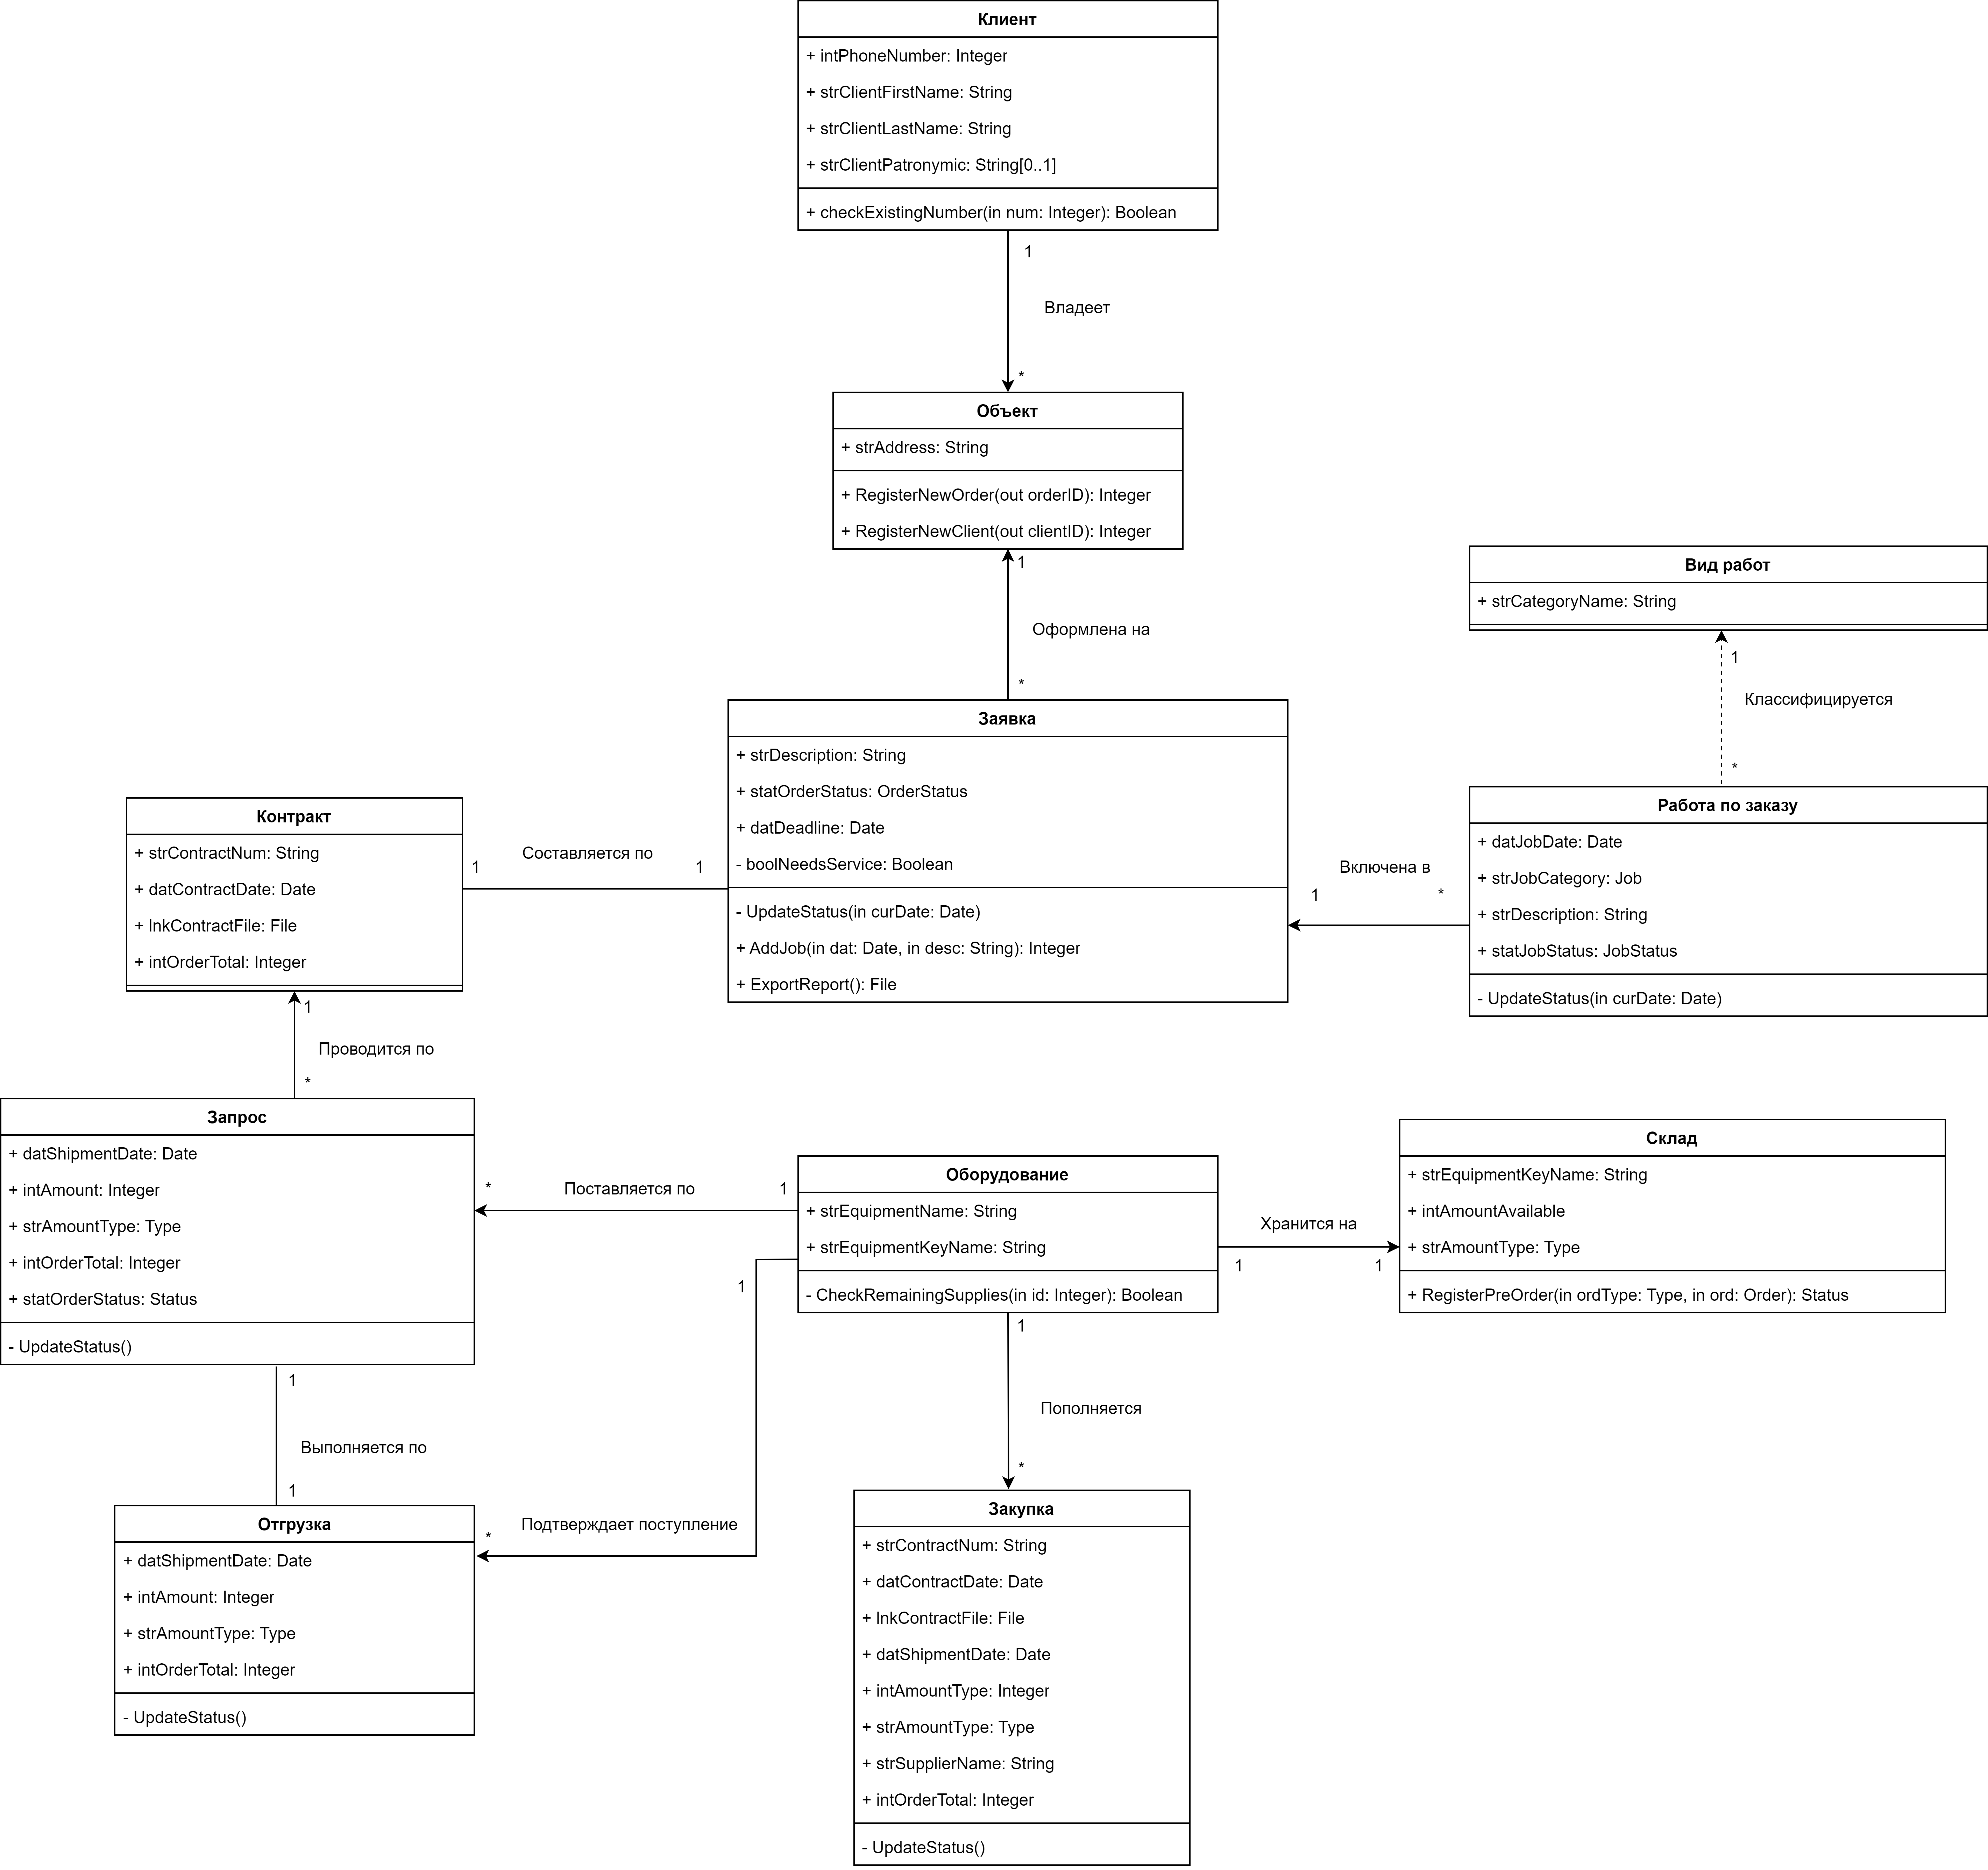
\includegraphics[width=\linewidth]{classes.png}
    \caption{Диаграмма классов АИС}
    \label{fig:classes}
\end{figure}

%%% Глава 2           %%%
%%%                   %%%
%%%%%%%%%%%%%%%%%%%%%%%%%



%%%%%%%%%%%%%%%%%%%%%%%%%
%%%                   %%%
%%% Глава 3           %%%

% \newpage
% \section{Глава 3}

%%% Глава 3           %%%
%%%                   %%%
%%%%%%%%%%%%%%%%%%%%%%%%%



%%%%%%%%%%%%%%%%%%%%%%%%%
%%%                   %%%
%%% Заключение        %%%

\newpage
\section*{Промежуточные итоги}
\addcontentsline{toc}{section}{Промежуточные итоги}

На данном этапе выполнены следующие задачи:
\begin{itemize}
    \item Провести обследование процессов предприятия Заказчика;
    \item Сформулировать техническое задание на разработку системы (частично).
\end{itemize}

В ходе практики по научно-исследовательской работе было выполнено обследование деятельности компании и сформулировано высокоуровневое техническое задание. Спецификация функций и реляционная модель базы данных будущей системы в значительной степени готовы, но не были включены в этот промежуточный отчет, поскольку еще требуют доработки.

Для завершения этой работы предстоит выполнить следующие шаги:
\begin{itemize}
    \item Создать макет дизайна автоматизированной системы;
    \item Разработать и протестировать программный код автоматизированной системы;
    \item Внедрить автоматизированную систему на предприятие заказчика;
    \item Исправить найденные в процессе эксплуатации недочеты.
\end{itemize}

Поддержка работы АИС будет выполняться после окончания практики по научно-исследовательской работе на протяжении всего использования автоматизированной системы Заказчиком.


%%% Заключение        %%%
%%%                   %%%
%%%%%%%%%%%%%%%%%%%%%%%%%



%%%%%%%%%%%%%%%%%%%%%%%%%
%%%                   %%%
%%% Литература        %%%

% \newpage
% \addcontentsline{toc}{section}{Список литературы}
% \bibliographystyle{plain}
% \bibliography{refs}

%%%  Литература       %%%
%%%                   %%%
%%%%%%%%%%%%%%%%%%%%%%%%%


%%%%%%%%%%%%%%%%%%%%%%%%%
%%%                   %%%
%%% Приложение        %%%

\newpage
\section*{Приложение}
\addcontentsline{toc}{section}{Приложение}

\begin{figure}[h]
    \centering
    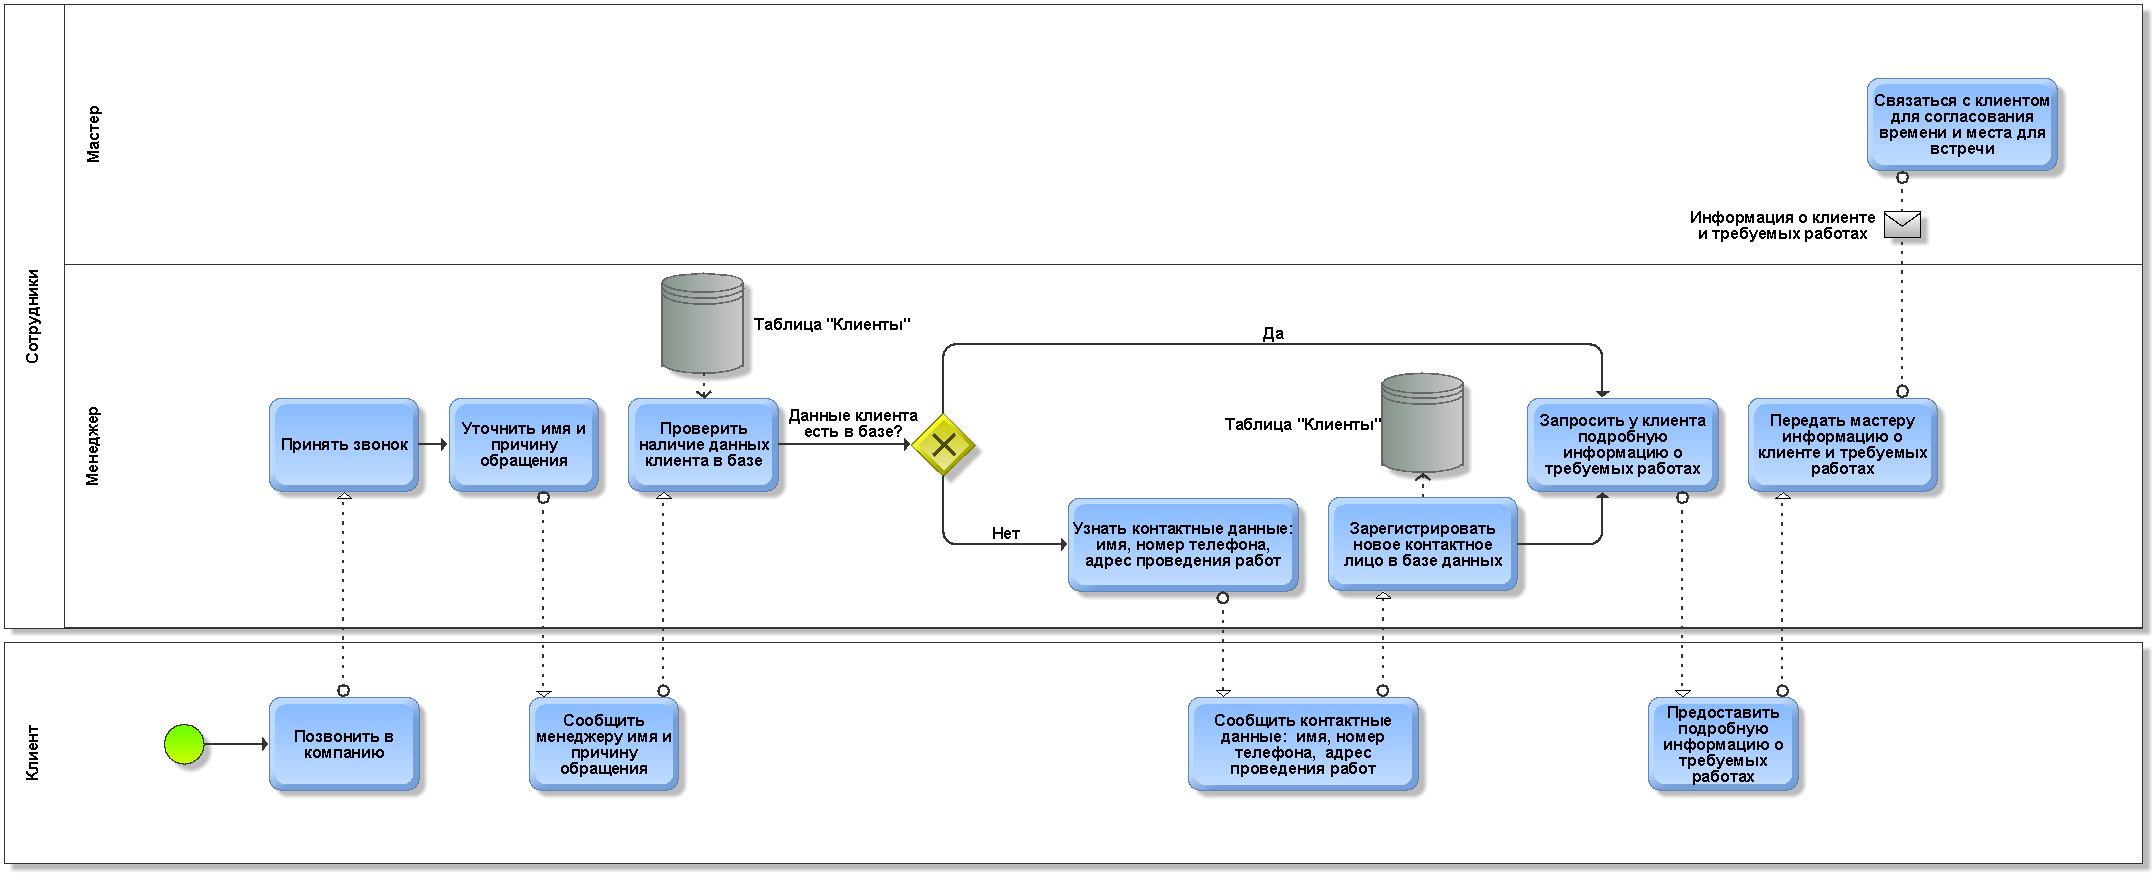
\includegraphics[width=\linewidth]{pred1.png}
    \caption{Диаграмма бизнес-процесса «Предпродажная работа»}
    \label{fig:pred1}
\end{figure}
\begin{figure}[h]
    \centering
    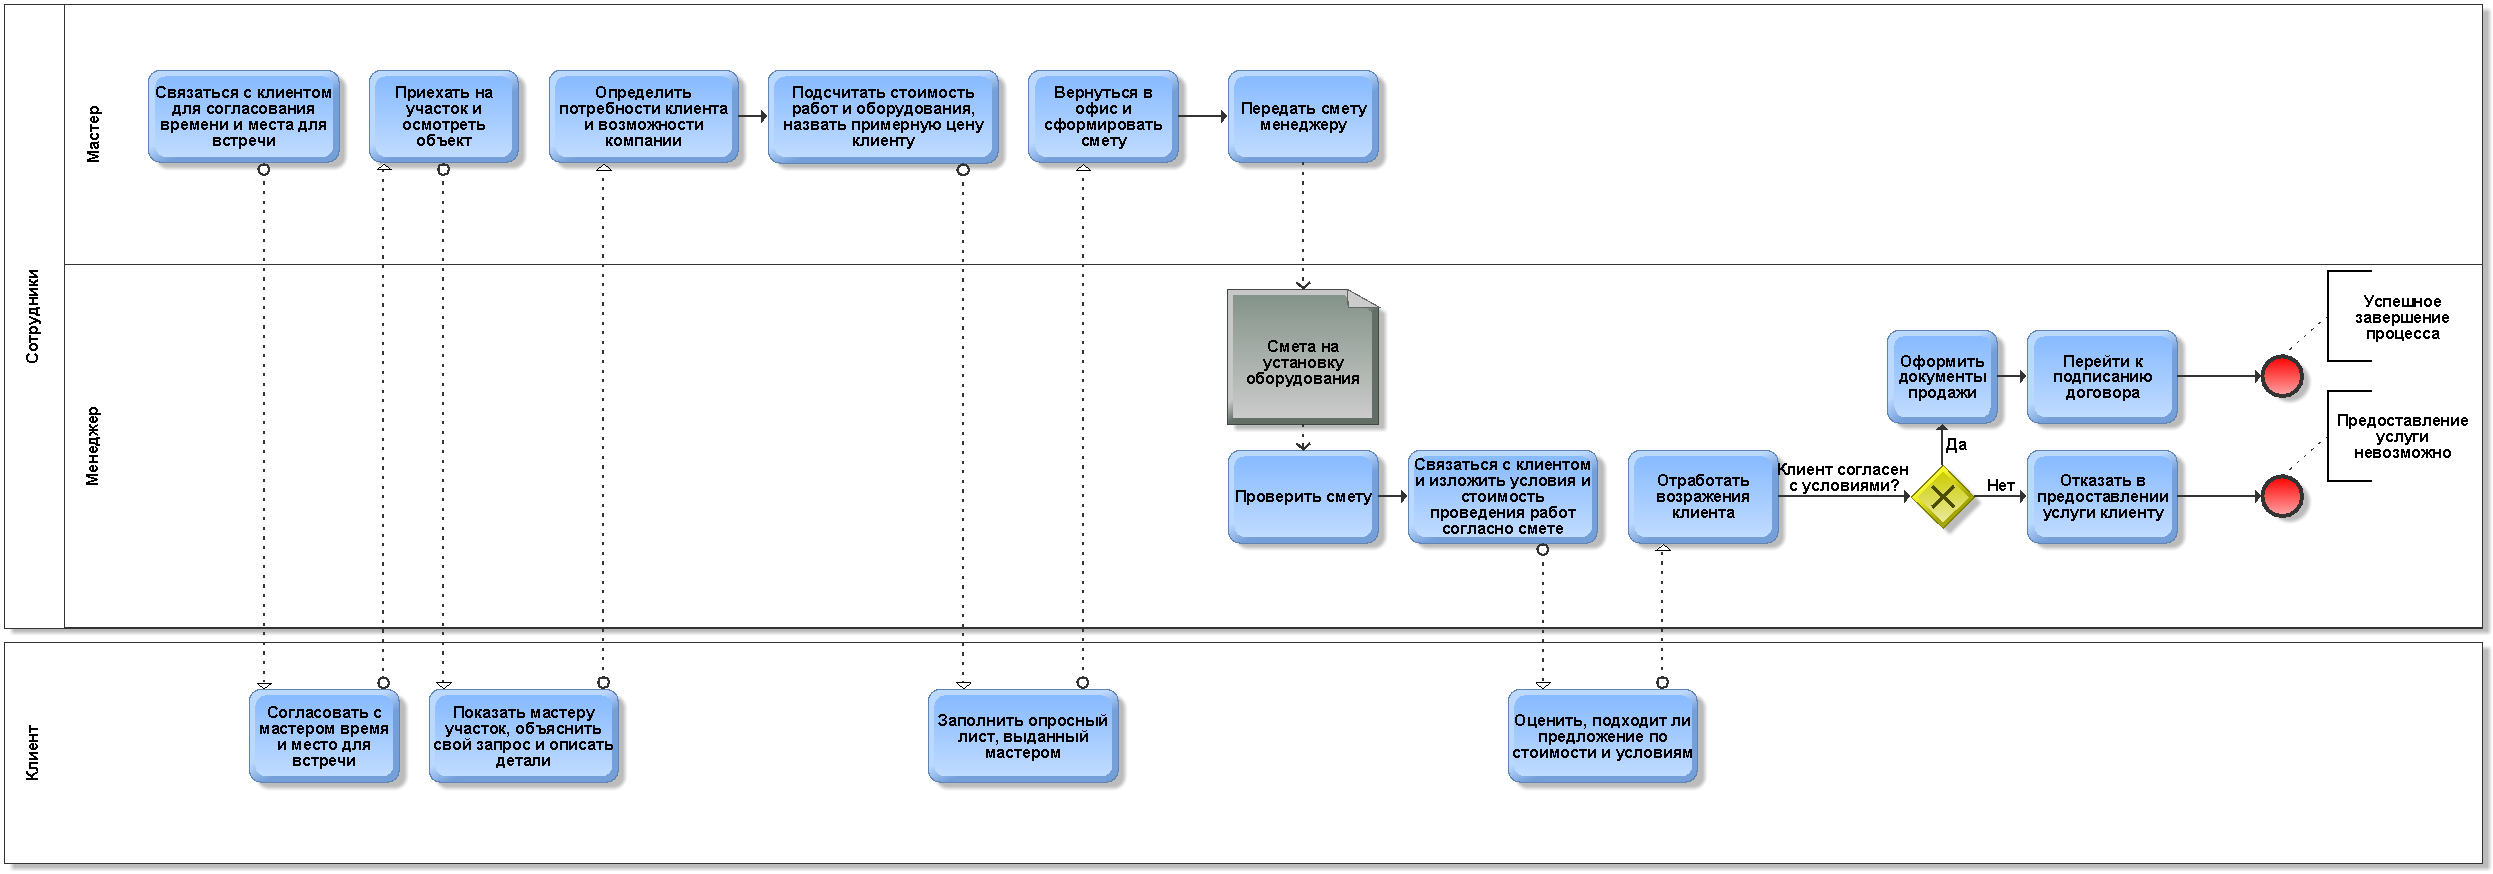
\includegraphics[width=\linewidth]{pred2.png}
    \caption{Диаграмма бизнес-процесса «Предпродажная работа» (продолжение)}
    \label{fig:pred2}
\end{figure}

\begin{figure}[h]
    \centering
    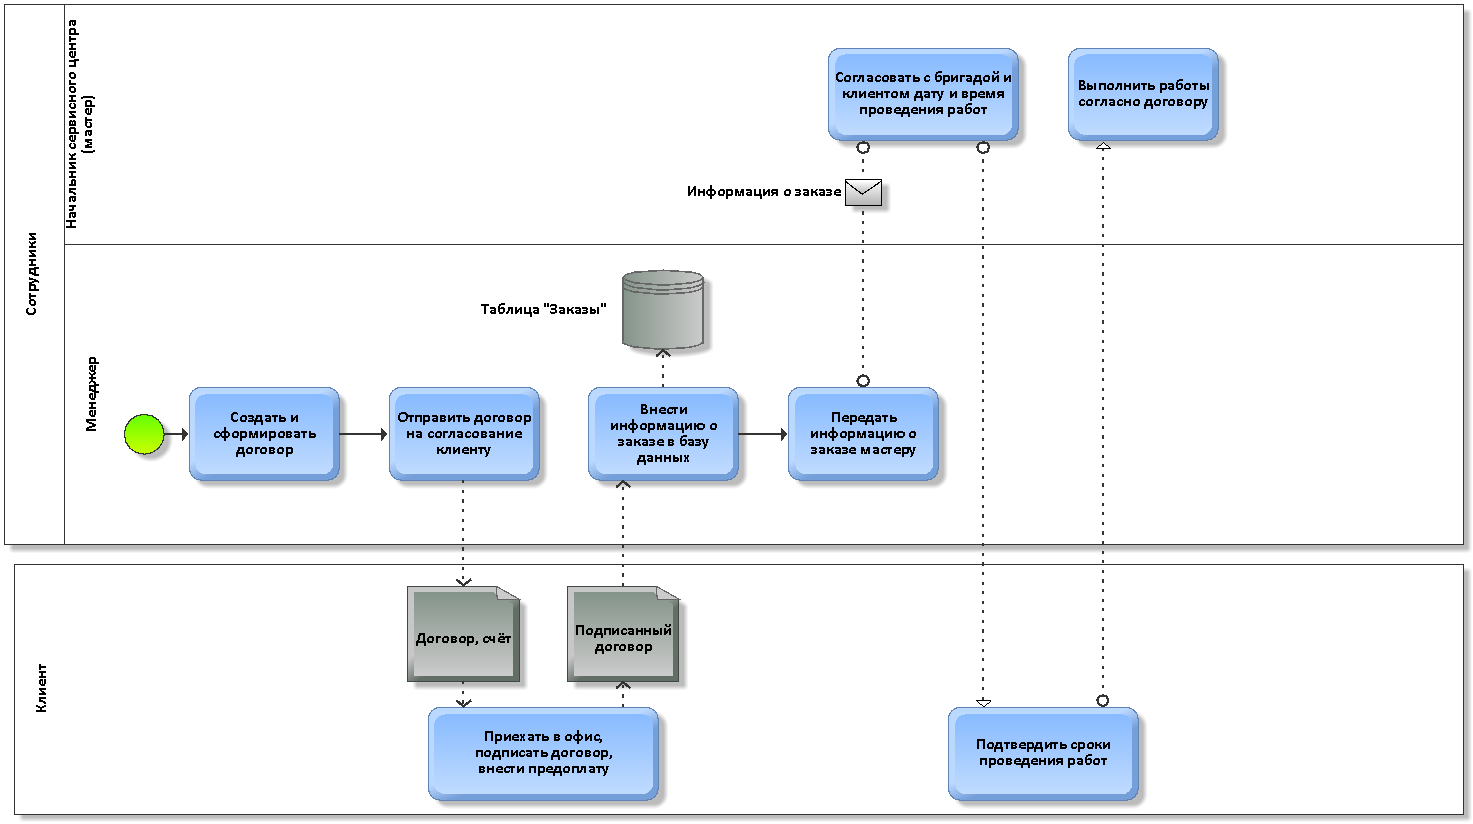
\includegraphics[width=\linewidth]{exec1.png}
    \caption{Диаграмма бизнес-процесса «Выполнение заказа клиента»}
    \label{fig:exec1}
\end{figure}
\begin{figure}[h]
    \centering
    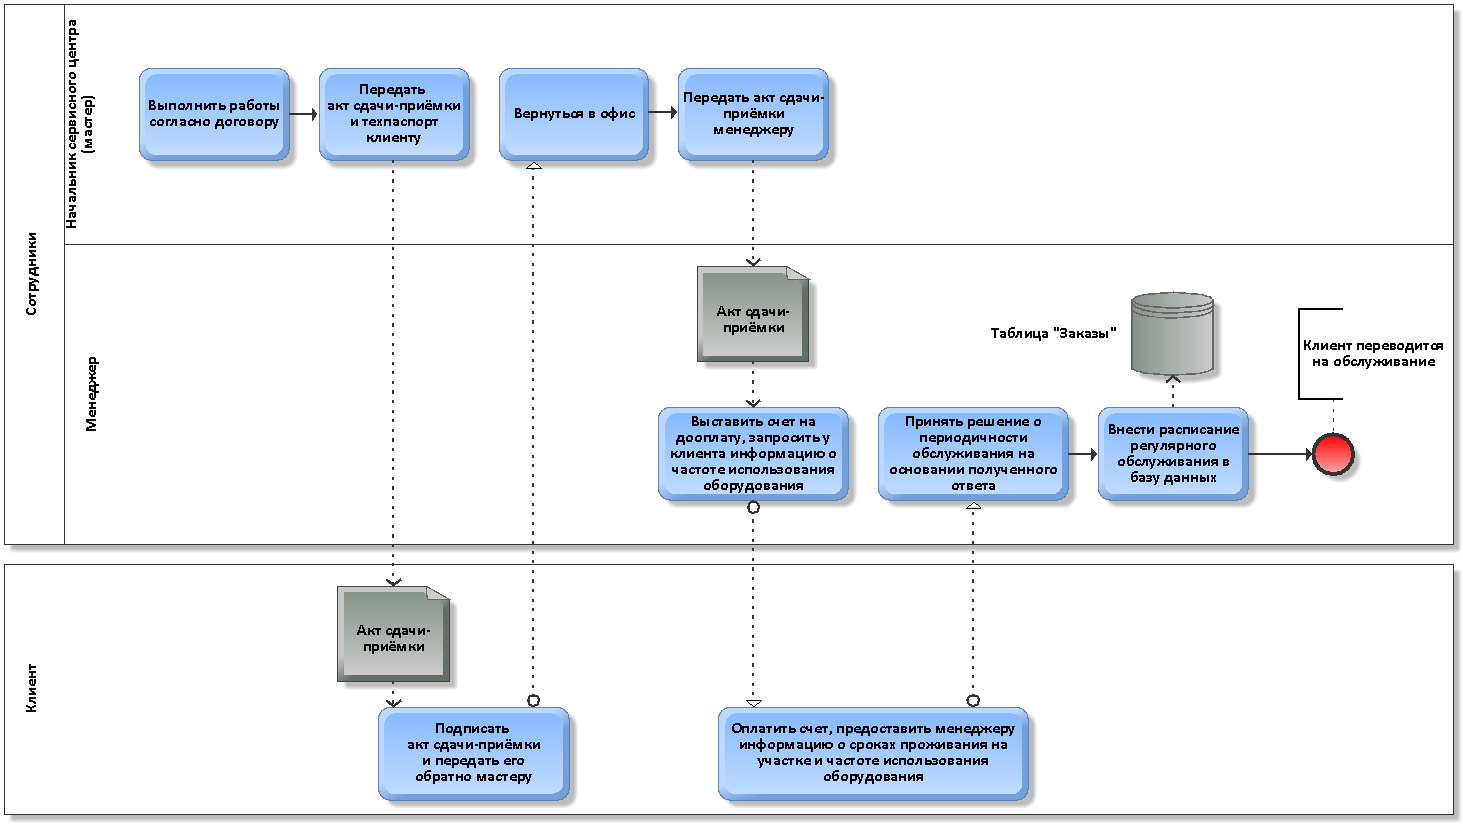
\includegraphics[width=\linewidth]{exec2.png}
    \caption{Диаграмма бизнес-процесса «Выполнение заказа клиента» (продолжение)}
    \label{fig:exec2}
\end{figure}

\begin{figure}[h]
    \centering
    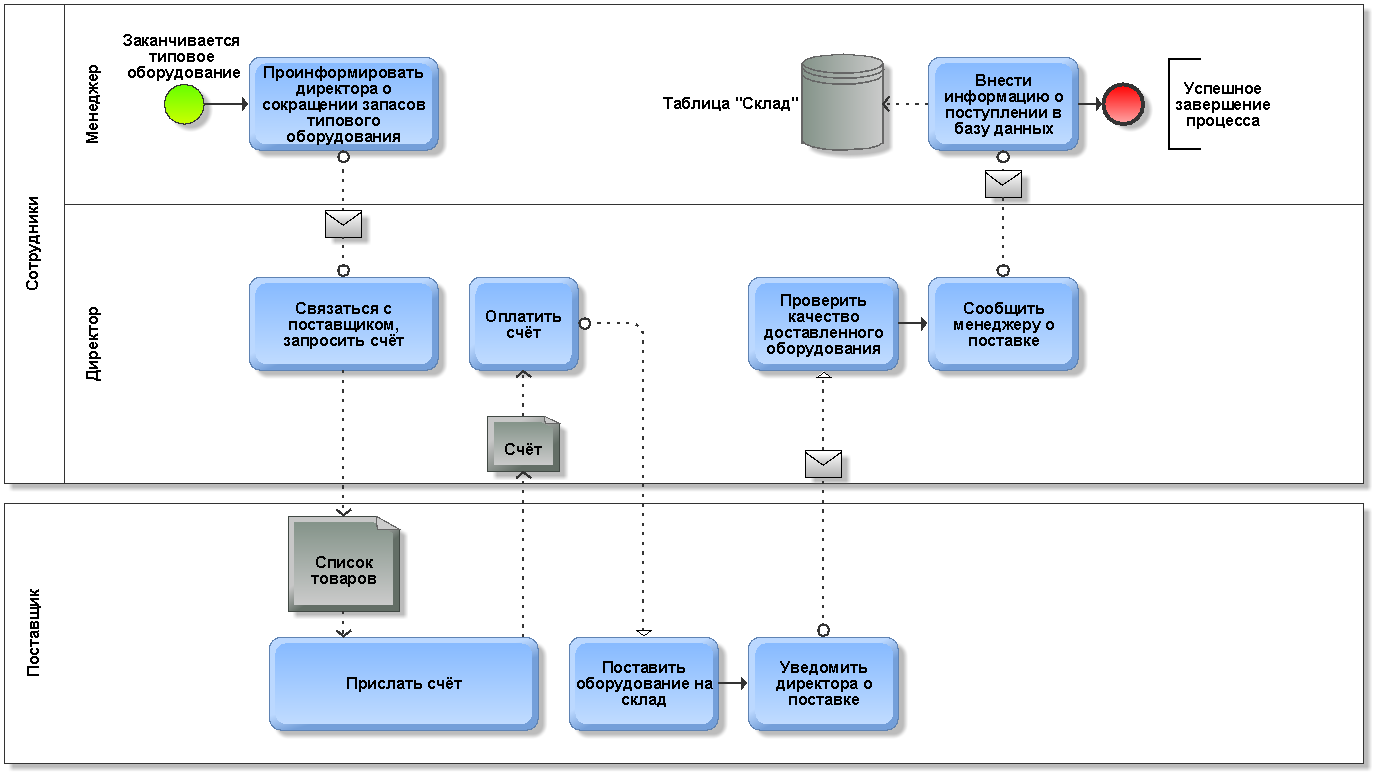
\includegraphics[width=\linewidth]{order1.png}
    \caption{Диаграмма бизнес-процесса «Заказ типового оборудования»}
    \label{fig:order1}
\end{figure}
\begin{figure}[h]
    \centering
    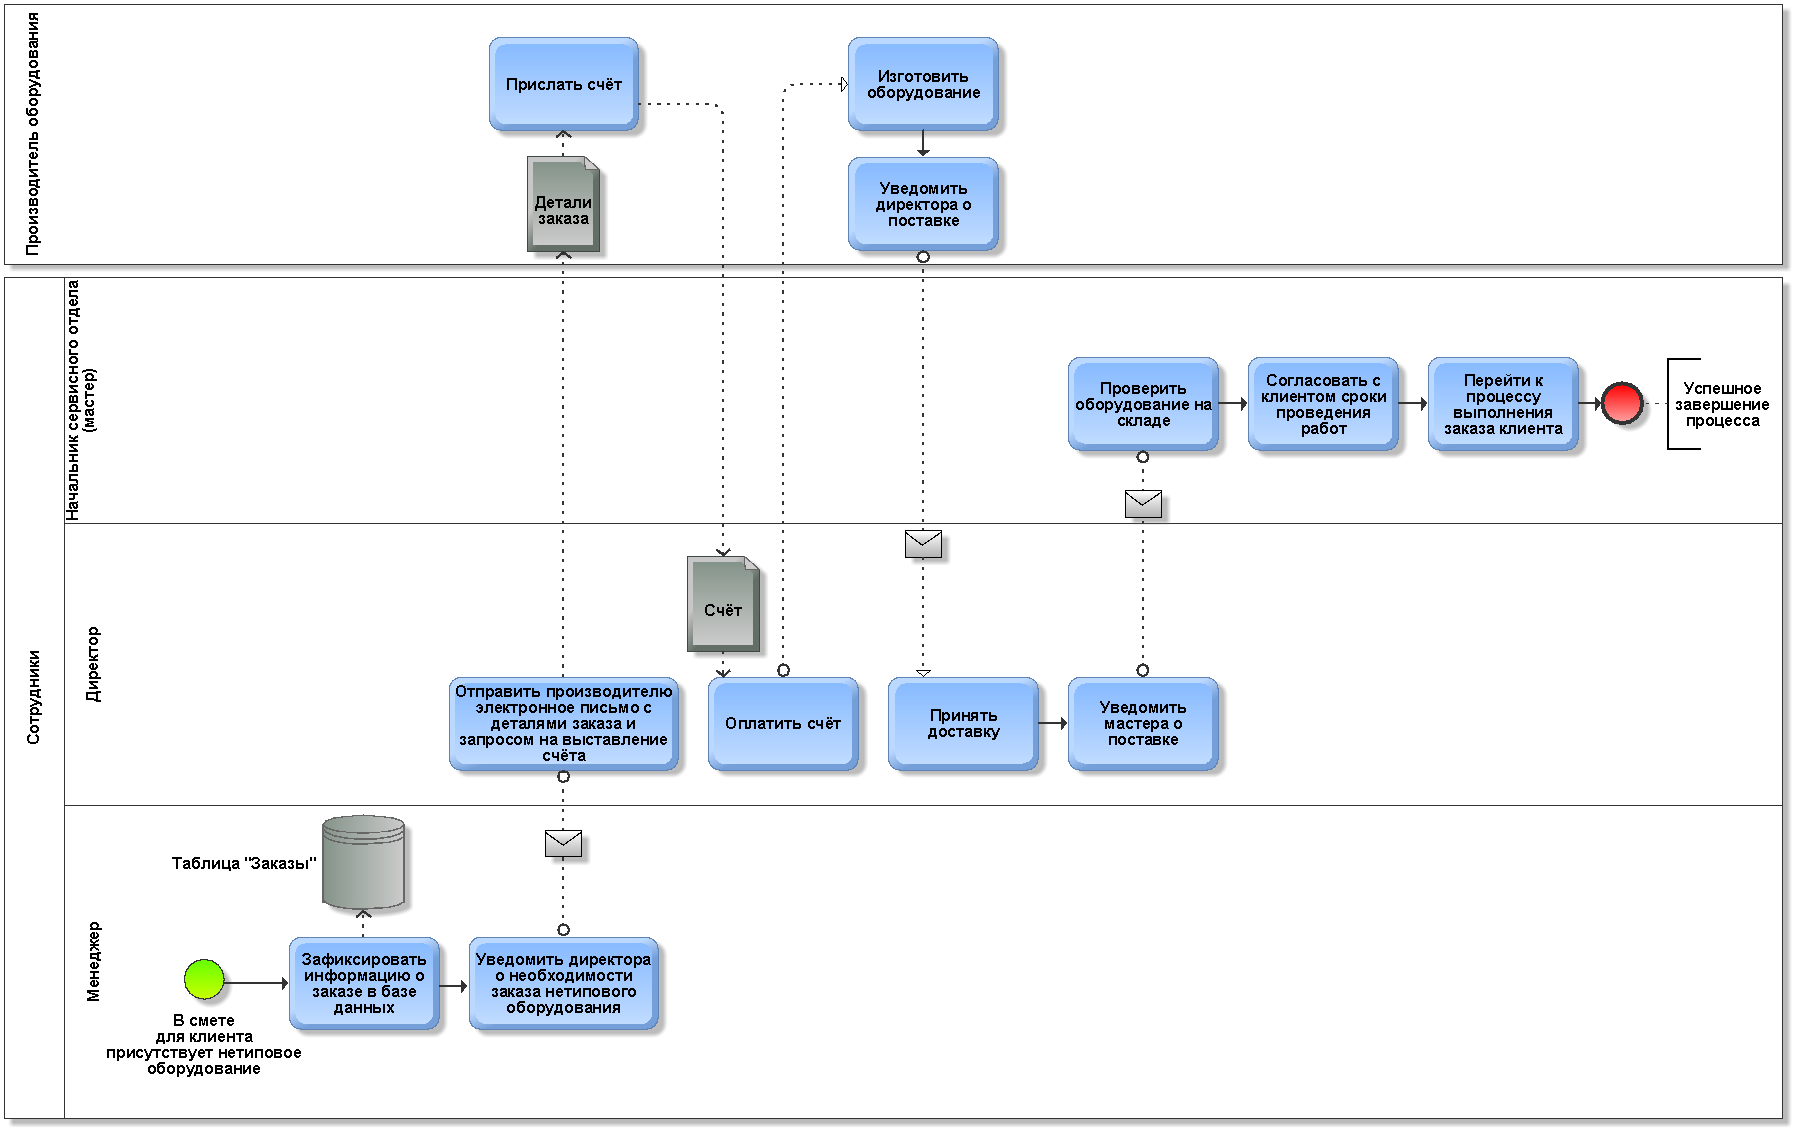
\includegraphics[width=\linewidth]{order2.png}
    \caption{Диаграмма бизнес-процесса «Заказ нетипового оборудования»}
    \label{fig:order2}
\end{figure}

\begin{figure}[h]
    \centering
    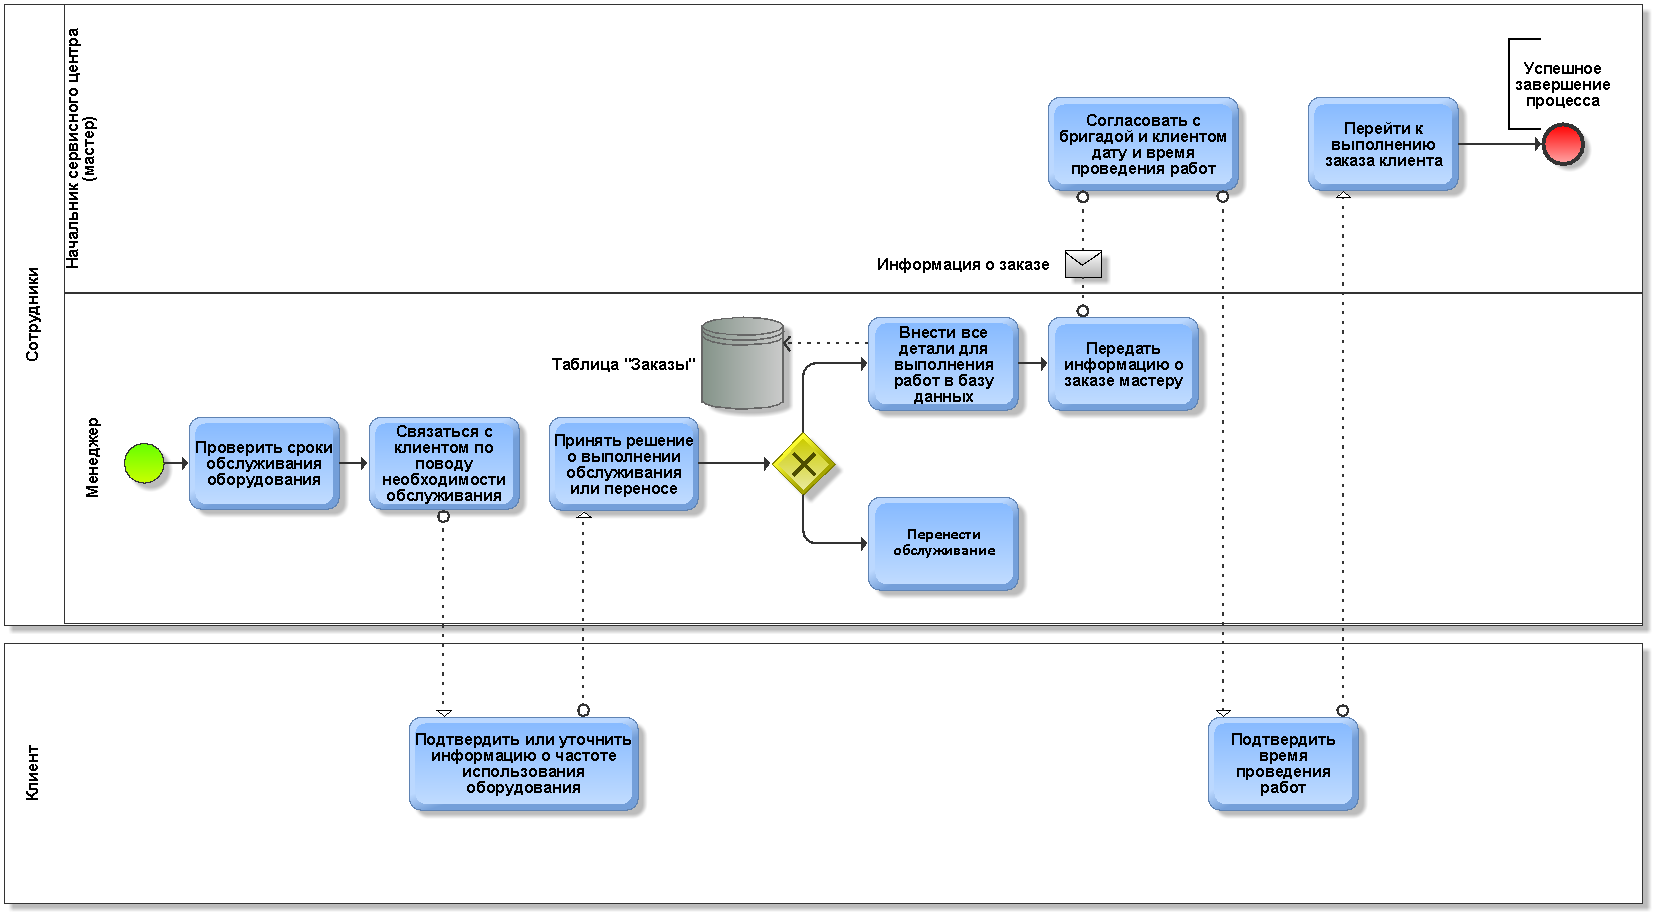
\includegraphics[width=\linewidth]{service.png}
    \caption{Диаграмма бизнес-процесса «Регулярное обслуживание оборудования»}
    \label{fig:service}
\end{figure}

%%% Приложение        %%%
%%%                   %%%
%%%%%%%%%%%%%%%%%%%%%%%%%
 

\end{document}